%!Tex Root = ../Tutorat4.tex
% ./Packete.tex
% ./Design.tex
% ./Deklarationen.tex
% ./Aufgabe1.tex
% ./Aufgabe3.tex
% ./Bonus.tex

\section{Task 2}

\setcounter{task}{1}

\begin{frame}[allowframebreaks]{Task 2}{Schedulability Test for Fixed Priorities – Rate Monotonic (RM)}
  % task 1
  \begin{tasknoinc}
    \begin{itemize}
      \item task-set schedulable with \alert{RM}
      \item using \alert{sufficient} test
    \end{itemize}
    \begin{NiceTabular}{X[1,c]X[2,c]X[2,c]X[2,c]}[rules/color=SecondaryColor] % {\linewidth}{|C|C|L|L|}
        \CodeBefore
        \chessboardcolors{white}{BoxColor}
        \rowcolor{SecondaryColor}{1}
        \columncolor{SecondaryColor}{1}
        \Body
        & \textcolor{white}{$\tau_1$} & \textcolor{white}{$\tau_2$} & \textcolor{white}{$\tau_3$} \\
        \textcolor{white}{$C_i$} & 1 & 3 & 2 \\
        \textcolor{white}{$T_i$} & 3 & 8 & 9 \\
        \bottomrule
      \end{NiceTabular}
  \end{tasknoinc}
  \begin{requirementsnoinc}
    \begin{itemize}
      \item $\displaystyle U=\sum_{i=1}^n \frac{C_i}{T_i} \leq n\left(2^{1 / n}-1\right)$, $U$ is the \alert{fraction} of the \alert{processor time} spent on \alert{executing task set }
    \end{itemize}
  \end{requirementsnoinc}
  \begin{solution}
    \begin{itemize}
      \item $\frac{1}{3} + \frac{3}{8} + \frac{2}{9} = 0.93 \le 3(2^{\frac{1}{3}} - 1) = 0.78$ \quad $\times$
      \item condition is \alert{not necessary}, hence we \alert{don’t know} whether the task set is schedulable with \alert{RM} or not
    \end{itemize}
  \end{solution}
  \framebreak
  % task 2
  \begin{tasknoinc}
    \begin{itemize}
      \item task-set schedulable with \alert{RM}
      \item using \alert{necessary} test
    \end{itemize}
    \begin{NiceTabular}{X[1,c]X[2,c]X[2,c]X[2,c]}[rules/color=SecondaryColor] % {\linewidth}{|C|C|L|L|}
        \CodeBefore
        \chessboardcolors{white}{BoxColor}
        \rowcolor{SecondaryColor}{1}
        \columncolor{SecondaryColor}{1}
        \Body
        & \textcolor{white}{$\tau_1$} & \textcolor{white}{$\tau_2$} & \textcolor{white}{$\tau_3$} \\
        \textcolor{white}{$C_i$} & 1 & 3 & 2 \\
        \textcolor{white}{$T_i$} & 3 & 8 & 9 \\
        \bottomrule
      \end{NiceTabular}
  \end{tasknoinc}
  \hspace{0.5cm}
  \begin{requirementsnoinc}
    \begin{itemize}
      \item guarantee that \alert{all} the tasks can be scheduled in \alert{any possible instance}
      \item in particular, if a task can be scheduled in its \alert{critical instances}, then the schedulability guarantee condition holds
      \begin{itemize}
        \item a \alert{critical instance} of a task occurs whenever the task is \alert{released simultaneously} with \alert{all higher priority tasks}
      \end{itemize}
      \item \alert{Schedulability Test:} For all tasks $\tau_i$ smallest $R_i$ that satisfies $\displaystyle R_i=C_i+\sum_{j=1}^{i-1}\left\lceil\frac{R_i}{T_j}\right\rceil C_j$ and $R_i \le D_i$ (necessary and sufficient)
    \end{itemize}
  \end{requirementsnoinc}
  \begin{requirementsnoinc}
    \begin{figure}
      \centering
      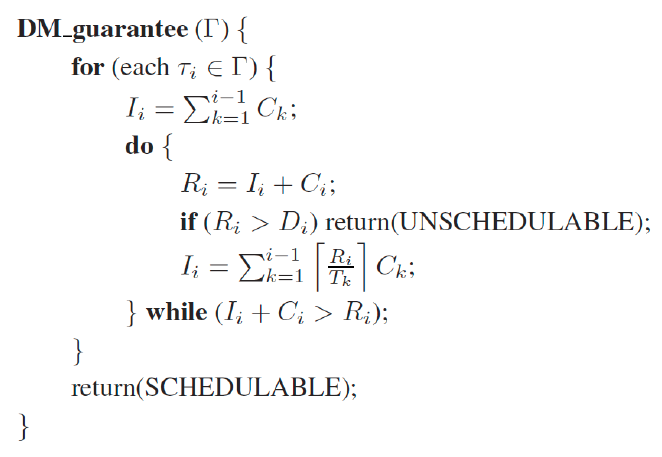
\includegraphics[height=0.5\paperheight]{./figures/2_algorithm.png}
    \end{figure}
  \end{requirementsnoinc}
  \begin{solutionnoinc}
    \begin{itemize}
      \item The tasks are first ordered by their priorities: $\tau_1$, $\tau_2$ and $\tau_3$
      \begin{itemize}
        \item In this case the tasks are already ordered
      \end{itemize}
      \item $\tau_3:$
      \begin{itemize}
        \item $R_3^0=1+3+2=6 \quad I_3^0=\left\lceil\frac{6}{3}\right\rceil 1+\left\lceil\frac{6}{8}\right\rceil 3=2+3=5 \quad 5+2 \le 6$ $\times$
        \item $R_3^1=5+2=7 \quad I_3^1=\left\lceil\frac{7}{3}\right\rceil 1+\left\lceil\frac{7}{8}\right\rceil 3=3+3=6 \quad 6+2 \le 7$ $\times$
        \item $R_3^2=6+2=8 \quad I_3^2=\left\lceil\frac{8}{3}\right\rceil 1+\left\lceil\frac{8}{8}\right\rceil 3=3+3=6 \quad 6+2 \le 8$ $\checkmark$

        $\Rightarrow R_3=8 \leq T_3=9$ $\checkmark$
      \end{itemize}
    \end{itemize}
  \end{solutionnoinc}
  \begin{solution}
    \begin{itemize}
      \item $\tau_2$:
        \begin{itemize}
          \item $R_2^0=1+3=4 \quad I_2^0=\left\lceil\frac{4}{3}\right\rceil 1=2 \quad 2+3 \le 4$ $\times$
          \item $R_2^1=2+3=5 \quad I_2^1=\left\lceil\frac{5}{3}\right\rceil 1=2 \quad 2+3 \leq 5$ $\checkmark$
        \end{itemize}

          $\Rightarrow R_2=5 \leq T_2=8$ $\checkmark$
      \item $\tau_1$:
      \begin{itemize}
        \item $R_1^0=C_1=1 \quad I_1^0=0 \quad 0+1\le 1$ $\checkmark$
      \end{itemize}

          $\Rightarrow R_1=1 \leq T_1=3$ $\checkmark$
      \item The necessary and sufficient test succeeds. This means that the task set is schedulable with RM.
    \end{itemize}
  \end{solution}
  \framebreak
  % task 3
  \begin{tasknoinc}
    \begin{itemize}
      \item first job of each task arrives at time $0$
      \item construct schedule for interval $[0, 20]$
    \end{itemize}
    \begin{NiceTabular}{X[1,c]X[2,c]X[2,c]X[2,c]}[rules/color=SecondaryColor] % {\linewidth}{|C|C|L|L|}
        \CodeBefore
        \chessboardcolors{white}{BoxColor}
        \rowcolor{SecondaryColor}{1}
        \columncolor{SecondaryColor}{1}
        \Body
        & \textcolor{white}{$\tau_1$} & \textcolor{white}{$\tau_2$} & \textcolor{white}{$\tau_3$} \\
        \textcolor{white}{$r_i$} & 0 & 0 & 0 \\
        \textcolor{white}{$C_i$} & 1 & 3 & 2 \\
        \textcolor{white}{$T_i$} & 3 & 8 & 9 \\
        \bottomrule
      \end{NiceTabular}
  \end{tasknoinc}
  \begin{solutionnoinc}
    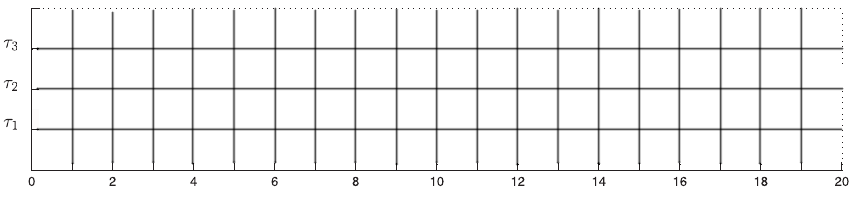
\includegraphics[width=\textwidth]{./figures/2_sol_empty.png}
  \end{solutionnoinc}
  \begin{solution}
    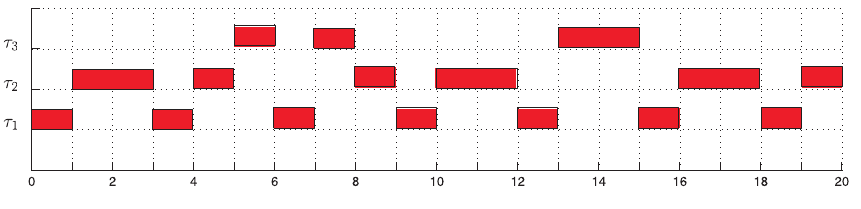
\includegraphics[width=\textwidth]{./figures/2_sol.png}
  \end{solution}
\end{frame}
